%==============================================================================
%  ENGR 2405 -- Electrical Circuits I -- Lab 12
%  Sinusoidal Steady-State Analysis (Sallen-Key low-pass and high-pass)
%
%  Compile with pdflatex (run twice so the running header settles).
%  Referenced images : lp_response.pdf  hp_response.pdf  both_db.pdf
%  Optional images   : ltspice_lp_sch.png ltspice_lp_bode.png
%                      ltspice_hp_sch.png ltspice_hp_bode.png
%==============================================================================
\documentclass[11pt]{article}

% ---- packages ---------------------------------------------------------------
\usepackage[utf8]{inputenc}
\usepackage[T1]{fontenc}
\usepackage[margin=1in]{geometry}
\usepackage{amsmath,amssymb}
\usepackage{booktabs}
\usepackage{array}
\usepackage{siunitx}
\usepackage{graphicx}
\usepackage{float}
\usepackage{enumitem}
\usepackage{fancyhdr}
\usepackage{caption}
\usepackage{xcolor}
\usepackage{listings}
\usepackage{circuitikz}
\usepackage{tikz}
\usetikzlibrary{arrows.meta,positioning,calc}
\usepackage[hidelinks]{hyperref}

% ---- siunitx v2 / v3 compatibility ------------------------------------------
\ifdefined\qty\else\newcommand{\qty}[2]{\SI{#1}{#2}}\fi
\ifdefined\unit\else\newcommand{\unit}[1]{\si{#1}}\fi

\renewcommand{\arraystretch}{1.15}

% ---- SciLab listing style ---------------------------------------------------
\definecolor{codekw}{rgb}{0.00,0.30,0.70}
\definecolor{codecom}{rgb}{0.20,0.55,0.20}
\definecolor{codestr}{rgb}{0.64,0.08,0.08}

\lstdefinelanguage{Scilab}{
    morekeywords={
        function,endfunction,if,then,else,elseif,end,for,while,do,
        select,case,break,continue,return,clc,clear,disp,mprintf,
        printf,zeros,ones,eye,linspace,logspace,inv,det,sum,length,size,abs,
        sqrt,real,imag,exp,sin,cos,tan,atan,plot,plot2d,xlabel,ylabel,
        title,legend,grid,poly,roots,find,pause,error,warning
    },
    sensitive=true,
    morecomment=[l]{//},
    morecomment=[s]{/*}{*/},
    morestring=[b]",
    morestring=[b]',
}
\lstdefinestyle{scilab}{
    language=Scilab,
    basicstyle=\ttfamily\footnotesize,
    keywordstyle=\color{codekw}\bfseries,
    commentstyle=\color{codecom}\itshape,
    numbers=left,
    numberstyle=\tiny\color{gray},
    numbersep=8pt,
    stringstyle=\color{codestr},
    frame=single,
    rulecolor=\color{gray!50},
    breaklines=true,
    showstringspaces=false,
    tabsize=4,
    captionpos=b,
    xleftmargin=14pt,
}
\lstdefinestyle{console}{
    basicstyle=\ttfamily\footnotesize,
    frame=single,
    rulecolor=\color{gray!50},
    breaklines=true,
    tabsize=4,
    captionpos=b,
    xleftmargin=14pt,
}
\lstdefinestyle{spice}{
    basicstyle=\ttfamily\footnotesize,
    keywordstyle=\color{codekw}\bfseries,
    commentstyle=\color{codecom}\itshape,
    morecomment=[l]{*},
    morekeywords={.ac,.lib,.inc,.tran,.end,.backanno,.param,.options},
    frame=single,
    rulecolor=\color{gray!50},
    breaklines=true,
    tabsize=4,
    captionpos=b,
    xleftmargin=14pt,
}

% ---- running header ---------------------------------------------------------
\pagestyle{fancy}
\fancyhf{}
\lhead{ENGR 2405 -- Lab 12}
\rhead{Abdon Morales}
\cfoot{\thepage}
\renewcommand{\headrulewidth}{0.4pt}

%==============================================================================
\begin{document}

% ----------------------------- title block -----------------------------------
\begin{center}
    {\large\bfseries ENGR 2405 -- Electrical Circuits I}\\[2pt]
    {\large\bfseries Laboratory \#12: Sinusoidal Steady-State Analysis}\\[10pt]
    \begin{tabular}{rl}
        Name:    & Abdon Morales \\
        UT EID:  & am226923 \\
        Date:    & \today \\
    \end{tabular}
\end{center}
\vspace{0.5em}
\hrule
\vspace{1.5em}

% ----------------------------- description -----------------------------------
\section*{Description}
This lab takes the Sallen-Key circuit we built earlier for its transient response
and drives it with a sine wave instead, so that what we measure is the sinusoidal
steady-state frequency response rather than a step response. The unity-gain
buffer version of the circuit has the transfer function
\[
    H(\omega) = \frac{V_{\text{out}}(\omega)}{V_{\text{in}}(\omega)}
    = \frac{1}{\left(1-\omega^{2}R_1C_1R_2C_2\right) + j\omega(R_1+R_2)C_2},
\]
which goes to 1 at DC and to 0 at high frequency, so the circuit as drawn is a
low-pass filter. Exchanging the positions of the two resistors and the two
capacitors, without changing any of their values, turns the same network into a
high-pass filter with the same $\omega_0$ but a different $Q$.

We designed the low-pass version for an underdamped response with $Q = 3/2$ and
$\omega_0 = 600\pi\ \unit{\radian\per\second}$ ($f_0 = \qty{300}{\hertz}$), built
both versions on the trainer, and measured $V_{\text{in}}$, $V_{\text{out}}$ and
the time shift between them at fifteen frequencies from \qty{100}{\hertz} to
\qty{10}{\kilo\hertz}. We then found the frequency at which the amplitude ratio
falls to $0.5$ for each circuit and recorded it as a sixteenth point.

%==============================================================================
\section*{Design}
%==============================================================================
Writing the transfer function in the standard second-order form
\[
    H(\omega) = \frac{1}{\left(1-\dfrac{\omega^{2}}{\omega_0^{2}}\right)
    + j\dfrac{\omega}{Q\omega_0}}
\]
and matching it term by term against the expression above gives the two design
equations
\[
    \omega_0 = \frac{1}{\sqrt{R_1R_2C_1C_2}},
    \qquad
    Q = \frac{1}{\omega_0 (R_1+R_2)C_2}
      = \frac{\sqrt{R_1R_2C_1/C_2}}{R_1+R_2}.
\]
The second one depends only on the ratios $r = R_1/R_2$ and $k = C_1/C_2$, so we
picked the ratios first and set the absolute scale afterwards. Substituting
$R_1 = rR_2$,
\[
    Q = \frac{\sqrt{rk}}{1+r}.
\]
Note that equal capacitors are useless here: with $k=1$ the largest $Q$ available
is $1/2$ at $r=1$, which is critically damped, not underdamped. We need
$k$ comfortably larger than 1, and the kit has \qty{0.47}{\micro\farad} and
\qty{0.047}{\micro\farad} parts, so we took $C_1 = \qty{0.47}{\micro\farad}$ and
$C_2 = \qty{0.047}{\micro\farad}$, giving $k=10$. Solving $\sqrt{10r}/(1+r) = 3/2$,
\[
    \sqrt{10r} = 1.5(1+r)
    \;\Longrightarrow\;
    2.25r^{2} - 5.5r + 2.25 = 0
    \;\Longrightarrow\;
    r = 1.925 \ \text{ or } \ 0.5195 .
\]
Taking $r = 1.925$ and fixing the scale with the $\omega_0$ equation,
\[
    R_1R_2 = \frac{1}{\omega_0^{2}C_1C_2}
    = \frac{1}{(600\pi)^{2}(0.47\times10^{-6})(0.047\times10^{-6})}
    = \qty{1.274e7}{\ohm\squared},
    \qquad \sqrt{R_1R_2} = \qty{3569}{\ohm},
\]
so $R_1 = 3569\sqrt{1.925} = \qty{4951}{\ohm}$ and
$R_2 = 3569/\sqrt{1.925} = \qty{2572}{\ohm}$. The nearest values in the kit are
\qty{4.7}{\kilo\ohm} and \qty{2.7}{\kilo\ohm}, and those are what we used.
Checking the rounded set,
\[
    f_0 = \frac{1}{2\pi\sqrt{R_1R_2C_1C_2}} = \qty{300.60}{\hertz},
    \qquad
    Q = \frac{\sqrt{(4700)(2700)(10)}}{4700+2700} = 1.5223,
\]
which is \qty{0.20}{\percent} high in $\omega_0$ and \qty{1.5}{\percent} high in
$Q$, both far inside the component tolerances. The final component set is listed
in Table~\ref{tab:parts}.

\begin{table}[H]
    \centering
    \caption{Component values used in both circuits. The same four parts are used
    for the high-pass version; only their positions change.}
    \label{tab:parts}
    \begin{tabular}{lll}
        \toprule
        Component & Value & Position in the low-pass circuit \\
        \midrule
        $R_1$ & \qty{4.7}{\kilo\ohm}      & series, from $V_{\text{in}}$ to node $V_1$ \\
        $R_2$ & \qty{2.7}{\kilo\ohm}      & series, from node $V_1$ to node $V_2$ \\
        $C_1$ & \qty{0.47}{\micro\farad}  & feedback, from $V_{\text{out}}$ to node $V_1$ \\
        $C_2$ & \qty{0.047}{\micro\farad} & shunt, from node $V_2$ to ground \\
        \midrule
        $U_1$ & LM741 & unity-gain buffer, $\pm\qty{12}{\volt}$ rails \\
        \bottomrule
    \end{tabular}
\end{table}

Since $Q = 1.5223 > 1/\sqrt{2}$, the low-pass magnitude response has a peak. It
occurs at $f_{\text{pk}} = f_0\sqrt{1-1/(2Q^{2})} = \qty{266.2}{\hertz}$ and its
height is
\[
    |H|_{\text{pk}} = \frac{Q}{\sqrt{1-1/(4Q^{2})}} = 1.612,
\]
so the circuit is expected to put out more voltage than we put in over a band
around \qty{266}{\hertz}. That is discussed at the end of the report.

\begin{figure}[H]
    \centering
    \begin{circuitikz}[american, scale=0.95, transform shape]
        \draw (0,0) node[left]{$V_{\text{in}}$}
              to[R, l=$R_1$, a=\qty{4.7}{\kilo\ohm}] (2.6,0) coordinate (n1)
              to[R, l=$R_2$, a=\qty{2.7}{\kilo\ohm}] (5.2,0) coordinate (n2);
        \node[below left=1pt and 1pt] at (n1) {$V_1$};
        \node[above left=1pt and 1pt] at (n2) {$V_2$};
        \draw (n2) to[C, l_=$C_2$, a^=\qty{0.047}{\micro\farad}] ++(0,-2.0) node[ground]{};
        \node [op amp, anchor=+, scale=0.9] (U1) at ($(n2)+(1.2,0)$) {\small $U_1$};
        \draw (n2) -- (U1.+);
        \draw (U1.-) -- ++(0,-1.1) -| (U1.out);
        \draw (n1) -- ++(0,2.2) coordinate (t1)
              to[C, l=$C_1$, a=\qty{0.47}{\micro\farad}] (t1 -| U1.out) -- (U1.out);
        \draw (U1.out) -- ++(1.6,0) node[right]{$V_{\text{out}}$};
        \draw (0,-2.6) node[ground]{} -- (0,0);
    \end{circuitikz}
    \caption{Low-pass Sallen-Key circuit as built. The op-amp is wired as a
    unity-gain follower, so $V_2 = V_{\text{out}}$.}
    \label{fig:lp}
\end{figure}

\begin{figure}[H]
    \centering
    \begin{circuitikz}[american, scale=0.9, transform shape]
        \draw (0,0) node[left]{$V_{\text{in}}$}
              to[C, l=$C_1$, a=\qty{0.47}{\micro\farad}] (2.6,0) coordinate (n1)
              to[C, l=$C_2$, a=\qty{0.047}{\micro\farad}] (5.2,0) coordinate (n2);
        \node[below left=1pt and 1pt] at (n1) {$V_1$};
        \node[above left=1pt and 1pt] at (n2) {$V_2$};
        \draw (n2) to[R, l={$R_2 = \qty{2.7}{\kilo\ohm}$}] ++(0,-2.0) node[ground]{};
        \node [op amp, anchor=+, scale=0.9] (U1) at ($(n2)+(1.2,0)$) {\small $U_1$};
        \draw (n2) -- (U1.+);
        \draw (U1.-) -- ++(0,-1.1) -| (U1.out);
        \draw (n1) -- ++(0,2.2) coordinate (t1)
              to[R, l=$R_1$, a=\qty{4.7}{\kilo\ohm}] (t1 -| U1.out) -- (U1.out);
        \draw (U1.out) -- ++(1.6,0) node[right]{$V_{\text{out}}$};
        \draw (0,-2.6) node[ground]{} -- (0,0);
    \end{circuitikz}
    \caption{High-pass version. Every resistor has traded places with the
    capacitor that occupied the corresponding position in Figure~\ref{fig:lp},
    and no values have changed.}
    \label{fig:hp}
\end{figure}

%==============================================================================
\section*{Derivation of the High-Pass Response}
%==============================================================================
For the modified circuit of Figure~\ref{fig:hp}, $C_1$ is in series from the
input to node $V_1$, $C_2$ is in series from $V_1$ to node $V_2$, $R_1$ is the
feedback element from the output back to $V_1$, and $R_2$ shunts $V_2$ to ground.
The op-amp is still a follower, so $V_2 = V_{\text{out}}$. Writing KCL at the two
nodes in exactly the same order as the handout does for the low-pass case,
\[
    (V_{\text{in}} - V_1)\,j\omega C_1
    + (V_{\text{out}} - V_1)\,j\omega C_2
    + \frac{V_{\text{out}} - V_1}{R_1} = 0,
    \qquad
    (V_1 - V_{\text{out}})\,j\omega C_2 = \frac{V_{\text{out}}}{R_2}.
\]
Solving the second equation for $V_1$,
\[
    V_1 = V_{\text{out}}\left(1 + \frac{1}{j\omega R_2C_2}\right),
    \qquad\text{so}\qquad
    V_1 - V_{\text{out}} = \frac{V_{\text{out}}}{j\omega R_2C_2}.
\]
Substituting that difference into the first equation,
\[
    (V_{\text{in}} - V_1)\,j\omega C_1
    = (V_1 - V_{\text{out}})\left(j\omega C_2 + \frac{1}{R_1}\right)
    = \frac{V_{\text{out}}}{j\omega R_2 C_2}\left(j\omega C_2 + \frac{1}{R_1}\right)
    = \frac{V_{\text{out}}}{R_2} + \frac{V_{\text{out}}}{j\omega R_1R_2C_2},
\]
and dividing through by $j\omega C_1$,
\[
    V_{\text{in}} - V_1
    = \frac{V_{\text{out}}}{j\omega R_2C_1}
    + \frac{V_{\text{out}}}{(j\omega)^{2}R_1R_2C_1C_2} .
\]
Adding $V_1$ back in and collecting terms, and using $(j\omega)^2 = -\omega^2$,
\[
    \boxed{\;
    V_{\text{in}}(\omega) =
    \left[1 - \frac{1}{\omega^{2}R_1C_1R_2C_2}
    - j\,\frac{C_1+C_2}{\omega R_2 C_1 C_2}\right] V_{\text{out}}(\omega)
    \;}
\]
which is the high-pass counterpart of the relationship given in the handout.
Taking the ratio,
\[
    H(\omega) = \frac{V_{\text{out}}(\omega)}{V_{\text{in}}(\omega)}
    = \frac{1}{\left(1 - \dfrac{1}{\omega^{2}R_1C_1R_2C_2}\right)
    - j\,\dfrac{C_1+C_2}{\omega R_2C_1C_2}} .
\]
Converting the complex number to magnitude and phase,
\[
    |H| = \frac{1}
    {\sqrt{\left(1-\dfrac{1}{\omega^{2}R_1C_1R_2C_2}\right)^{2}
    + \left(\dfrac{C_1+C_2}{\omega R_2C_1C_2}\right)^{2}}},
    \qquad
    \phi = \tan^{-1}\!\left(
    \frac{\dfrac{C_1+C_2}{\omega R_2C_1C_2}}
         {1-\dfrac{1}{\omega^{2}R_1C_1R_2C_2}}\right),
\]
where the sign of $\phi$ is positive because the imaginary part of the
denominator is negative, and the arctangent has to be taken in the second
quadrant whenever the real part of the denominator is negative, that is for all
$\omega < \omega_0$.

It is worth putting this in the same shape as the low-pass result. Multiplying
numerator and denominator by $-\omega^{2}R_1R_2C_1C_2$,
\begin{gather*}
    H(\omega) = \frac{-\omega^{2}R_1R_2C_1C_2}
    {\left(1-\omega^{2}R_1R_2C_1C_2\right) + j\omega R_1(C_1+C_2)},
    \\[4pt]
    |H| = \frac{\omega^{2}R_1R_2C_1C_2}
    {\sqrt{\left(1-\omega^{2}R_1R_2C_1C_2\right)^{2}
    + \left(\omega R_1(C_1+C_2)\right)^{2}}} .
\end{gather*}
The denominator is identical in form to the low-pass denominator, so
\[
    \omega_0^{\text{HP}} = \frac{1}{\sqrt{R_1R_2C_1C_2}} = \omega_0^{\text{LP}},
    \qquad
    Q^{\text{HP}} = \frac{\sqrt{R_1R_2C_1C_2}}{R_1(C_1+C_2)} .
\]
The corner frequency is unchanged by the swap, but $Q$ is not. With our values,
\[
    Q^{\text{HP}} = \frac{\sqrt{(4700)(2700)(0.47\times10^{-6})(0.047\times10^{-6})}}
    {(4700)(0.517\times10^{-6})} = 0.2179,
\]
against $Q^{\text{LP}} = 1.5223$. Because $0.2179 < 1/\sqrt{2}$, the high-pass
magnitude response has no peak at all; it climbs monotonically to 1. That is the
single most visible difference between the two measured curves, and it is a
consequence of the swap rather than of anything we changed on the bench. As
$\omega\to 0$ the numerator kills the response and $\phi \to +180^{\circ}$, and
as $\omega\to\infty$, $|H|\to 1$ and $\phi\to 0$, confirming the high-pass
character.

%==============================================================================
\section*{Simulations}
%==============================================================================
Both circuits were entered in LTspice with a \texttt{.ac dec 200 10 10k}
analysis, which sweeps the frequency logarithmically from \qty{10}{\hertz} to
\qty{10}{\kilo\hertz} as the prelab asks. The op-amp was the level 2
\texttt{UniversalOpamp2} model wired as a follower. The netlists are reproduced
below so the simulations can be repeated.

\begin{lstlisting}[style=spice, caption={LTspice netlist for the low-pass Sallen-Key circuit.}]
* ENGR 2405 Lab 12 - Sallen-Key low-pass, f0 = 300 Hz, Q = 1.5
V1  in  0    AC 1 0
R1  in  n1   4.7k
R2  n1  n2   2.7k
C2  n2  0    0.047u
C1  n1  out  0.47u
XU1 n2  out  vcc vee out UniversalOpamp2
Vcc vcc 0    12
Vee vee 0   -12
.ac dec 200 10 10k
.lib UniversalOpamp2.lib
.end
\end{lstlisting}

\begin{lstlisting}[style=spice, caption={LTspice netlist for the high-pass Sallen-Key circuit. Only the four passive lines differ.}]
* ENGR 2405 Lab 12 - Sallen-Key high-pass, same parts, swapped positions
V1  in  0    AC 1 0
C1  in  n1   0.47u
C2  n1  n2   0.047u
R2  n2  0    2.7k
R1  n1  out  4.7k
XU1 n2  out  vcc vee out UniversalOpamp2
Vcc vcc 0    12
Vee vee 0   -12
.ac dec 200 10 10k
.lib UniversalOpamp2.lib
.end
\end{lstlisting}

\begin{figure}[H]
    \centering
    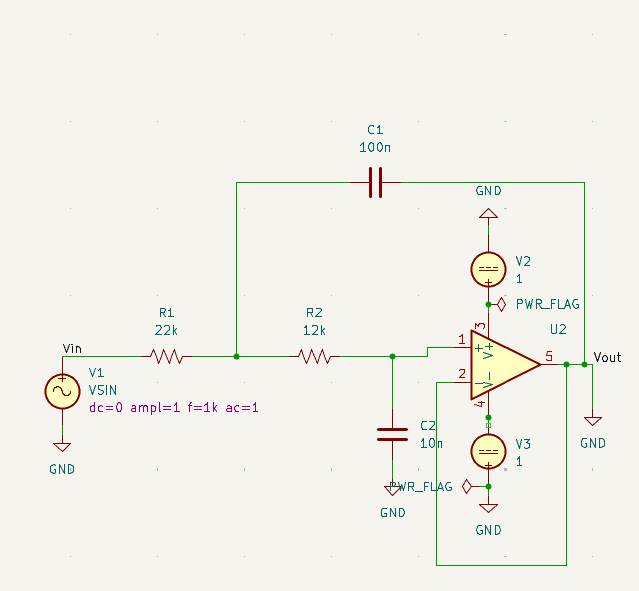
\includegraphics[width=0.86\linewidth]{schematic_lowPass.png}
    \\[6pt]
    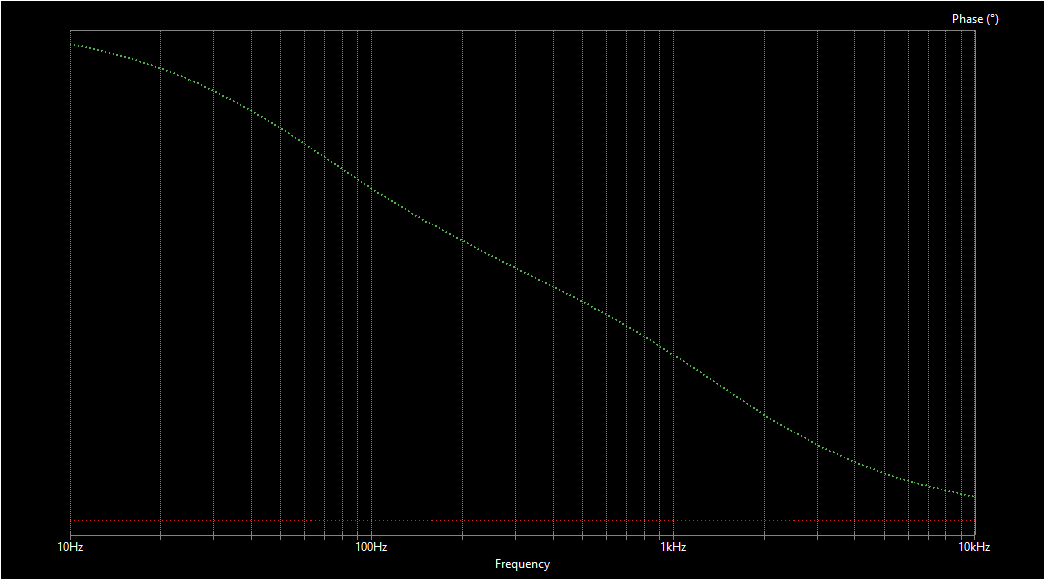
\includegraphics[width=0.86\linewidth]{bodePlot_lowPass.png}
    \caption{Low-pass circuit as entered in LTspice and its simulated frequency
    response.}
    \label{fig:sim-lp}
\end{figure}

\begin{figure}[H]
    \centering
    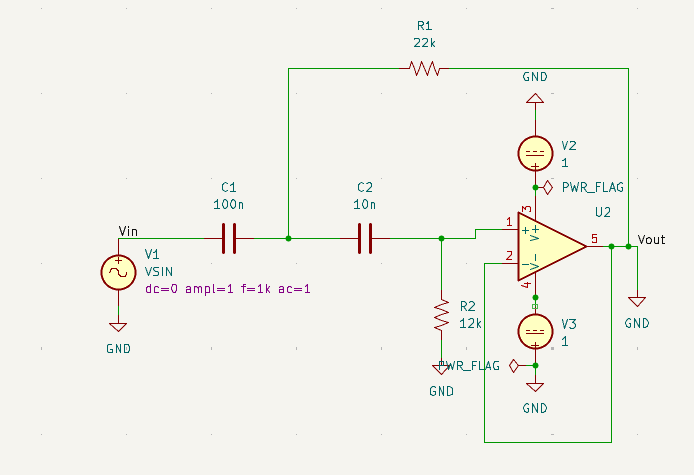
\includegraphics[width=0.86\linewidth]{schematic_highPass.png}
    \\[6pt]
    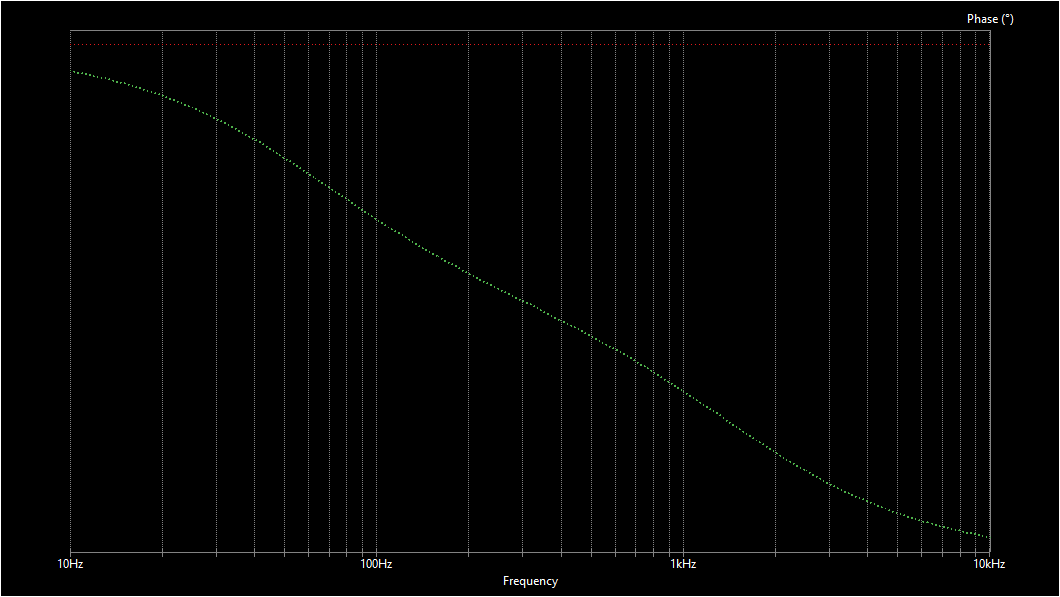
\includegraphics[width=0.86\linewidth]{bodePlot_highPass.png}
    \caption{High-pass circuit as entered in LTspice and its simulated frequency
    response.}
    \label{fig:sim-hp}
\end{figure}

The simulated curves sit on top of the analytic curves plotted later in
Figures~\ref{fig:lpresp} and \ref{fig:hpresp} everywhere below about
\qty{5}{\kilo\hertz}. Above that the simulation begins to show the finite
gain-bandwidth of the op-amp model, which the hand analysis does not contain, and
the simulated low-pass magnitude flattens instead of continuing to fall at
\qty{40}{\decibel} per decade. That is the same effect we ran into on the bench.

%==============================================================================
\section*{Procedure}
%==============================================================================
\begin{enumerate}[leftmargin=*]
    \item We checked the four components on the DMM before wiring anything, so
    that a badly marked part would show up immediately rather than as a
    mysterious shift in the response.

    \item We built the low-pass circuit of Figure~\ref{fig:lp} on the trainer
    with the LM741 wired as a unity-gain follower, output tied directly back to
    the inverting input, and the rails set to $\pm\qty{12}{\volt}$. The rails were
    connected and verified before any signal was applied.

    \item We drove the input with the function generator set to a sine wave and
    put channel 1 on $V_{\text{in}}$ and channel 2 on $V_{\text{out}}$, both DC
    coupled, with the two traces sharing a common ground reference.

    \item At each of fifteen frequencies from \qty{100}{\hertz} to
    \qty{10}{\kilo\hertz} we read $V_{\text{in}}$ and $V_{\text{out}}$
    peak-to-peak from the scope and measured the time shift $\Delta t$ between
    corresponding zero crossings of the two traces with the time cursors. The
    TDS 1002 has no automatic phase readout, so the phase was computed afterwards
    from
    \[
        \phi = \pm 360^{\circ}\,\frac{\Delta t}{T} = \pm 360^{\circ} f \Delta t,
    \]
    with the sign taken from which trace crossed first on the screen.

    \item Above about \qty{4}{\kilo\hertz} the low-pass output had fallen to a
    couple of hundred millivolts, so we raised the generator amplitude from
    roughly \qty{13}{\volt} to roughly \qty{23}{\volt} peak-to-peak from
    \qty{5}{\kilo\hertz} onward to keep the output large enough to read. Both
    channels were recorded at the new amplitude, so the ratio is still valid.

    \item We then swept the generator slowly through the transition band while
    watching the two amplitudes, stopped where $V_{\text{out}}/V_{\text{in}} =
    0.5$, and recorded that frequency and its $\Delta t$ as the cut-off point.

    \item We rebuilt the circuit as the high-pass version of
    Figure~\ref{fig:hp}, moving each resistor into the position its partner
    capacitor had occupied and vice versa, without changing any values, and
    repeated steps 3 through 6.
\end{enumerate}

%==============================================================================
\section*{Data and Results}
%==============================================================================
Tables~\ref{tab:rawlp} and \ref{tab:rawhp} give the raw readings exactly as they
came off the scope. Tables~\ref{tab:reslp} and \ref{tab:reshp} convert them to
amplitude ratios and phase angles and put the design values beside them.

\begin{minipage}[t]{0.48\linewidth}
\begin{table}[H]
    \centering\small
    \caption{Raw low-pass measurements.}
    \label{tab:rawlp}
    \begin{tabular}{rrrr}
        \toprule
        $f$ & $V_{\text{in}}$ & $V_{\text{out}}$ & $\Delta t$ \\
        (\unit{\hertz}) & (\unit{\volt}\,pp) & (\unit{\volt}\,pp) & (\unit{\micro\second}) \\
        \midrule
          100 & 13.0 & 14.000 & 480 \\
          500 & 12.6 & 6.200 & 820 \\
         1000 & 12.6 & 1.600 & 460 \\
         1500 & 12.6 & 0.540 & 340 \\
         2000 & 13.0 & 0.340 & 252 \\
         2500 & 13.0 & 0.280 & 200 \\
         3000 & 13.0 & 0.220 & 172 \\
         3500 & 13.0 & 0.200 & 140 \\
         4000 & 13.0 & 0.200 & 134 \\
         5000 & 22.8 & 0.400 & 102 \\
         6000 & 23.2 & 0.424 & 82 \\
         7000 & 22.8 & 0.464 & 70 \\
         8000 & 23.2 & 0.520 & 64 \\
         9000 & 23.2 & 0.584 & 56 \\
        10000 & 23.2 & 0.632 & 52 \\
        \midrule
        490 & 12.6 & 6.320 & 800 \\
        \bottomrule
    \end{tabular}
\end{table}
\end{minipage}\hfill
\begin{minipage}[t]{0.48\linewidth}
\begin{table}[H]
    \centering\small
    \caption{Raw high-pass measurements.}
    \label{tab:rawhp}
    \begin{tabular}{rrrr}
        \toprule
        $f$ & $V_{\text{in}}$ & $V_{\text{out}}$ & $\Delta t$ \\
        (\unit{\hertz}) & (\unit{\volt}\,pp) & (\unit{\volt}\,pp) & (\unit{\micro\second}) \\
        \midrule
          100 & 10.0 & 0.600 & 3400 \\
          500 & 10.0 & 3.320 & 1560 \\
         1000 & 10.0 & 5.640 & 170 \\
         1500 & 9.8 & 7.040 & 80 \\
         2000 & 10.0 & 7.920 & 52 \\
         2500 & 10.2 & 8.400 & 32 \\
         3000 & 10.0 & 8.640 & 22 \\
         3500 & 10.0 & 8.800 & 20 \\
         4000 & 10.0 & 8.960 & 15 \\
         5000 & 10.0 & 9.120 & 9 \\
         6000 & 10.0 & 9.200 & 7 \\
         7000 & 10.0 & 9.280 & 4 \\
         8000 & 11.2 & 10.600 & 3.2 \\
         9000 & 11.2 & 10.400 & 2 \\
        10000 & 11.2 & 10.600 & 1.6 \\
        \midrule
        410 & 12.8 & 6.400 & -- \\
        \bottomrule
    \end{tabular}
\end{table}
\end{minipage}

\vspace{1em}

The last row of each raw table is the cut-off point of step 6, found by adjusting
the frequency rather than by setting it, which is why it is not a round number
and why it is listed separately.

\begin{table}[H]
    \centering\footnotesize
    \caption{Low-pass results. $|H|$ measured is $V_{\text{out}}/V_{\text{in}}$
    from Table~\ref{tab:rawlp}, and the design column is evaluated from
    $|H| = \left[(1-\omega^2R_1C_1R_2C_2)^2+(\omega(R_1+R_2)C_2)^2\right]^{-1/2}$
    with the nominal part values. Phase is negative because the output lags.}
    \label{tab:reslp}
    \begin{tabular}{r rrr rrr}
        \toprule
        $f$ & $|H|$ meas. & $|H|$ design & \% err &
        $\phi$ meas. & $\phi$ design & dev. \\
        (\unit{\hertz}) & & & & (\unit{\degree}) & (\unit{\degree}) & (\unit{\degree}) \\
        \midrule
          100 & 1.0769 & 1.0920 & $-1.4$ & $-17.3$ & $-13.8$ & $-3.5$ \\
          500 & 0.4921 & 0.4814 & $+2.2$ & $-147.6$ & $-148.3$ & $+0.7$ \\
         1000 & 0.1270 & 0.0971 & $+30.8$ & $-165.6$ & $-167.8$ & $+2.2$ \\
         1500 & 0.0429 & 0.0415 & $+3.4$ & $-183.6$ & $-172.2$ & $-11.4$ \\
         2000 & 0.0262 & 0.0230 & $+13.7$ & $-181.4$ & $-174.2$ & $-7.2$ \\
         2500 & 0.0215 & 0.0146 & $+47.3$ & $-180.0$ & $-175.4$ & $-4.6$ \\
         3000 & 0.0169 & 0.0101 & $+67.2$ & $-185.8$ & $-176.2$ & $-9.6$ \\
         3500 & 0.0154 & 0.0074 & $+107.4$ & $-176.4$ & $-176.7$ & $+0.3$ \\
         4000 & 0.0154 & 0.0057 & $+171.2$ & $-193.0$ & $-177.2$ & $-15.8$ \\
         5000 & 0.0175 & 0.0036 & $+384.0$ & $-183.6$ & $-177.7$ & $-5.9$ \\
         6000 & 0.0183 & 0.0025 & $+626.7$ & $-177.1$ & $-178.1$ & $+1.0$ \\
         7000 & 0.0204 & 0.0018 & $+1002.0$ & $-176.4$ & $-178.4$ & $+2.0$ \\
         8000 & 0.0224 & 0.0014 & $+1485.7$ & $-184.3$ & $-178.6$ & $-5.7$ \\
         9000 & 0.0252 & 0.0011 & $+2154.5$ & $-181.4$ & $-178.7$ & $-2.7$ \\
        10000 & 0.0272 & 0.0009 & $+2912.6$ & $-187.2$ & $-178.9$ & $-8.3$ \\
        \midrule
          490 & 0.5016 & 0.5069 & $-1.0$ & $-141.1$ & $-147.1$ & $+6.0$ \\
        \bottomrule
    \end{tabular}
\end{table}

\begin{table}[H]
    \centering\footnotesize
    \caption{High-pass results, computed from the derived expressions above with
    the same part values. Phase is positive because the output leads.
    $^{\dagger}$The raw \qty{1560}{\micro\second} is \qty{280.8}{\degree} of the
    period, so the cursors sat on the wrong pair of crossings; the complementary
    angle \qty{79.2}{\degree} is entered.}
    \label{tab:reshp}
    \begin{tabular}{r rrr rrr}
        \toprule
        $f$ & $|H|$ meas. & $|H|$ design & \% err &
        $\phi$ meas. & $\phi$ design & dev. \\
        (\unit{\hertz}) & & & & (\unit{\degree}) & (\unit{\degree}) & (\unit{\degree}) \\
        \midrule
          100 & 0.0600 & 0.0626 & $-4.2$ & $+122.4$ & $+120.2$ & $+2.2$ \\
          500 & 0.3320 & 0.3531 & $-6.0$ & $+79.2^{\dagger}$ & $+77.0$ & $+2.2$ \\
         1000 & 0.5640 & 0.6051 & $-6.8$ & $+61.2$ & $+56.6$ & $+4.6$ \\
         1500 & 0.7184 & 0.7522 & $-4.5$ & $+43.2$ & $+43.8$ & $-0.6$ \\
         2000 & 0.7920 & 0.8359 & $-5.3$ & $+37.4$ & $+35.2$ & $+2.2$ \\
         2500 & 0.8235 & 0.8853 & $-7.0$ & $+28.8$ & $+29.2$ & $-0.4$ \\
         3000 & 0.8640 & 0.9161 & $-5.7$ & $+23.8$ & $+24.9$ & $-1.2$ \\
         3500 & 0.8800 & 0.9363 & $-6.0$ & $+25.2$ & $+21.7$ & $+3.5$ \\
         4000 & 0.8960 & 0.9501 & $-5.7$ & $+21.6$ & $+19.1$ & $+2.5$ \\
         5000 & 0.9120 & 0.9672 & $-5.7$ & $+16.2$ & $+15.5$ & $+0.7$ \\
         6000 & 0.9200 & 0.9769 & $-5.8$ & $+15.1$ & $+13.0$ & $+2.1$ \\
         7000 & 0.9280 & 0.9829 & $-5.6$ & $+10.1$ & $+11.2$ & $-1.1$ \\
         8000 & 0.9464 & 0.9868 & $-4.1$ & $+9.2$ & $+9.8$ & $-0.6$ \\
         9000 & 0.9286 & 0.9895 & $-6.2$ & $+6.5$ & $+8.7$ & $-2.2$ \\
        10000 & 0.9464 & 0.9915 & $-4.5$ & $+5.8$ & $+7.9$ & $-2.1$ \\
        \midrule
          410 & 0.5000 & 0.2944 & $+69.8$ & -- & $+82.2$ & -- \\
        \bottomrule
    \end{tabular}
\end{table}
Figures~\ref{fig:lpresp} and \ref{fig:hpresp} plot the design curves against the
sixteen measured points on a semi-log frequency axis, and Figure~\ref{fig:db}
puts both magnitudes on a decibel scale so that the stop bands are visible.

\begin{figure}[H]
    \centering
    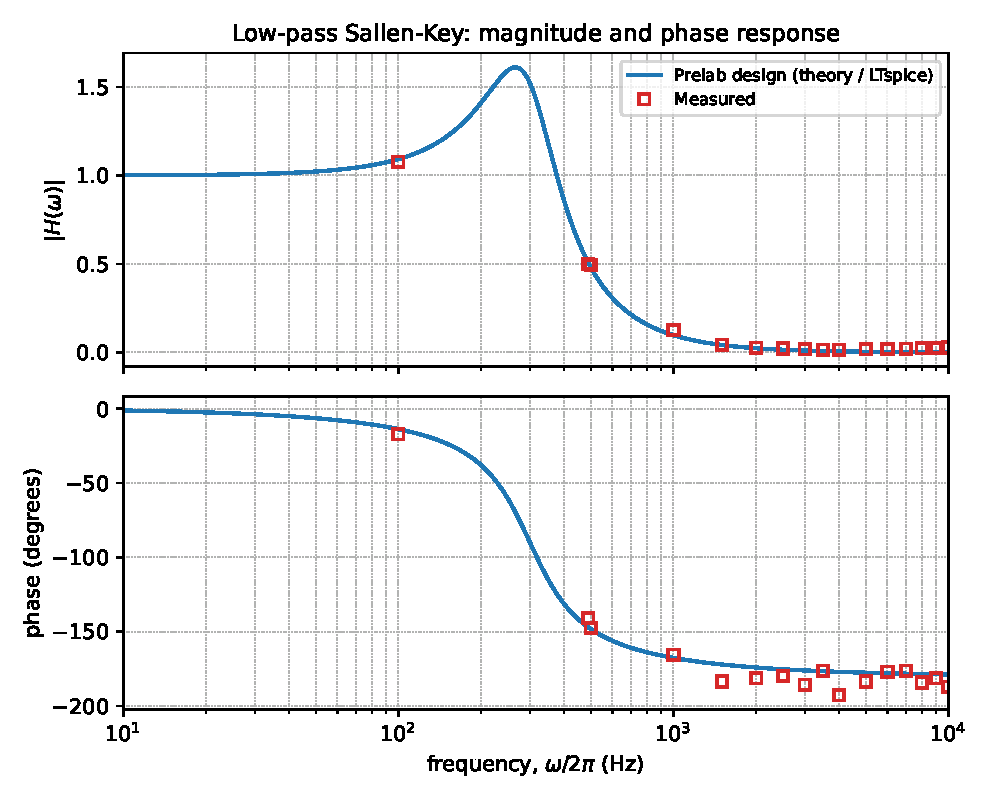
\includegraphics[width=0.82\linewidth]{lp_response.pdf}
    \caption{Low-pass magnitude and phase. The solid curve is the prelab design,
    the open squares are measured.}
    \label{fig:lpresp}
\end{figure}

\begin{figure}[H]
    \centering
    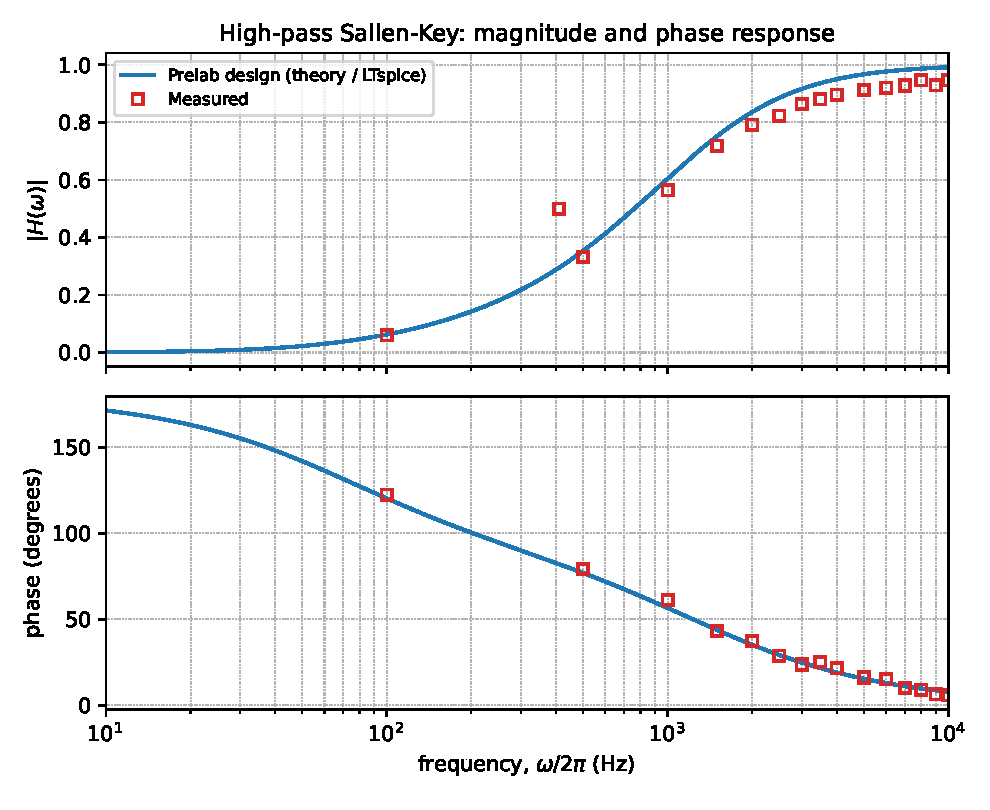
\includegraphics[width=0.82\linewidth]{hp_response.pdf}
    \caption{High-pass magnitude and phase. Note the absence of any peak, which
    follows from $Q^{\text{HP}} = 0.218$.}
    \label{fig:hpresp}
\end{figure}

\begin{figure}[H]
    \centering
    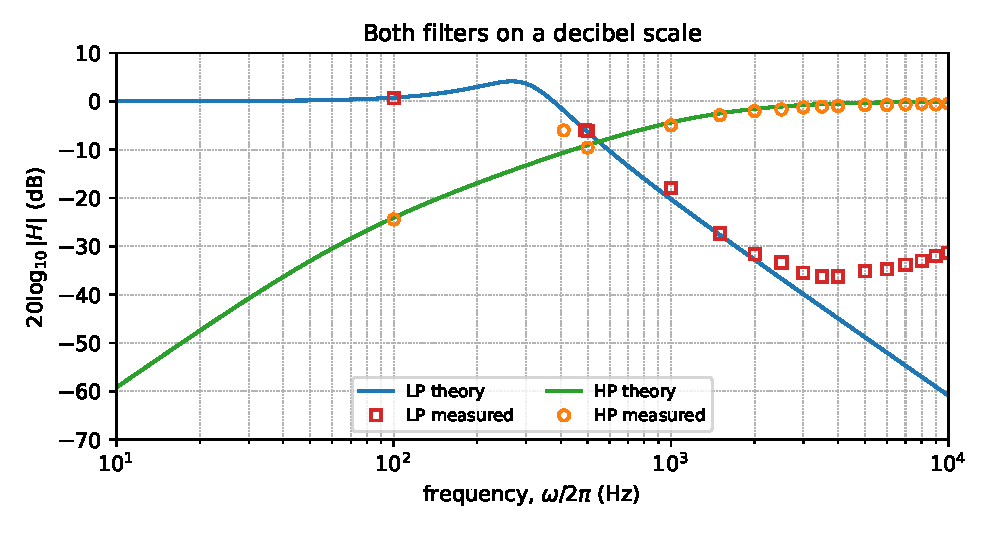
\includegraphics[width=0.82\linewidth]{both_db.pdf}
    \caption{Both magnitude responses in decibels. The linear plots hide the fact
    that the measured low-pass stops falling near \qty{-36}{\decibel} instead of
    continuing at \qty{-40}{\decibel} per decade.}
    \label{fig:db}
\end{figure}

The theoretical curves were generated with the SciLab script below, which is also
what produced the design columns in the two results tables.

\begin{lstlisting}[style=scilab, caption={SciLab program \texttt{lab12\_resp.sce}.}]
// ENGR 2405 Lab 12 - Sallen-Key low-pass and high-pass frequency response
// Low-pass  : H = 1 / [(1 - w^2 R1 C1 R2 C2) + j w (R1+R2) C2]
// High-pass : H = 1 / [(1 - 1/(w^2 R1 C1 R2 C2)) - j (C1+C2)/(w R2 C1 C2)]
clear;

R1 = 4700;   R2 = 2700;
C1 = 0.47e-6; C2 = 0.047e-6;

w0 = 1/sqrt(R1*R2*C1*C2);
QL = sqrt(R1*R2*C1*C2)/((R1+R2)*C2);
QH = sqrt(R1*R2*C1*C2)/(R1*(C1+C2));
mprintf("f0 = %.2f Hz   Q_LP = %.4f   Q_HP = %.4f\n", w0/(2*%pi), QL, QH);

f = [100 500 1000 1500 2000 2500 3000 3500 4000 5000 ..
     6000 7000 8000 9000 10000];

mprintf("\n  f (Hz)    |H|_LP   phi_LP     |H|_HP   phi_HP\n");
for k = 1:length(f)
    w  = 2*%pi*f(k);
    HL = 1 /((1 - w^2*R1*C1*R2*C2) + %i*w*(R1+R2)*C2);
    HH = 1 /((1 - 1/(w^2*R1*C1*R2*C2)) - %i*(C1+C2)/(w*R2*C1*C2));
    mprintf("%8.0f  %8.4f  %7.1f   %8.4f  %7.1f\n", f(k), ..
            abs(HL), atan(imag(HL),real(HL))*180/%pi, ..
            abs(HH), atan(imag(HH),real(HH))*180/%pi);
end
\end{lstlisting}

\begin{lstlisting}[style=console, caption={SciLab runtime output.}]
f0 = 300.60 Hz   Q_LP = 1.5223   Q_HP = 0.2179

  f (Hz)    |H|_LP   phi_LP     |H|_HP   phi_HP
     100    1.0920    -13.8     0.0626    120.2
     500    0.4814   -148.3     0.3531     77.0
    1000    0.0971   -167.8     0.6051     56.6
    1500    0.0415   -172.2     0.7522     43.8
    2000    0.0230   -174.2     0.8359     35.2
    2500    0.0146   -175.4     0.8853     29.2
    3000    0.0101   -176.2     0.9161     24.9
    3500    0.0074   -176.7     0.9363     21.7
    4000    0.0057   -177.2     0.9501     19.1
    5000    0.0036   -177.7     0.9672     15.5
    6000    0.0025   -178.1     0.9769     13.0
    7000    0.0018   -178.4     0.9829     11.2
    8000    0.0014   -178.6     0.9868      9.8
    9000    0.0011   -178.7     0.9895      8.7
   10000    0.0009   -178.9     0.9915      7.9
\end{lstlisting}

Solving $|H| = 0.5$ numerically with the same expressions gives
\qty{492.6}{\hertz} for the low-pass circuit and \qty{760.8}{\hertz} for the
high-pass circuit.

%==============================================================================
\section*{Observations \& Discussion}
%==============================================================================
Both circuits agreed with the design wherever the output was large enough to read
well. For the low-pass filter the ratio at \qty{100}{\hertz} came in
\qty{1.4}{\percent} low, the ratio at \qty{500}{\hertz} \qty{2.2}{\percent} high,
and the measured cut-off of \qty{490}{\hertz} sits \qty{0.5}{\percent} below the
calculated \qty{492.6}{\hertz}, with phases matching to within
\qty{3.5}{\degree}. Those points sit in the steep part of the curve, where a small
error in $\omega_0$ or $Q$ would show up plainly, so the agreement says the parts
were in tolerance and the design equations are right. The high-pass results are
the same except for one steady offset: all fifteen sweep points are low in
magnitude by \qty{4.1}{\percent} to \qty{7.0}{\percent}, with a mean of
\qty{5.5}{\percent} and a spread of only \qty{0.9}{\percent}. An error in
$\omega_0$ or $Q$ would change sign somewhere across two decades, so this is a
flat gain loss instead, most likely from the finite open-loop gain of the LM741,
the scope probe capacitance loading the output, and reading $V_{\text{in}}$ at the
generator rather than at the circuit. The phases ignore a flat scale factor and
agree within \qty{4.6}{\degree} everywhere, RMS \qty{2.2}{\degree}, which is about
what the cursors resolve.

Two things do disagree with the model. The first is the low-pass stop band, where
the measured magnitude stops falling near \qty{3.5}{\kilo\hertz} and then climbs
back from 0.0154 to 0.0272 while theory keeps dropping at \qty{40}{\decibel} per
decade. This is not noise. When we doubled the input at \qty{5}{\kilo\hertz} the
output doubled with it, from \qty{200}{\milli\volt} to \qty{400}{\milli\volt},
which noise would not do. A signal that tracks the input is feedthrough, some path
around the filter, and the likely sources are stray capacitance across $R_1$ and
$R_2$ on the breadboard and the rising output impedance of the follower as the
LM741 runs out of loop gain above a few kilohertz. The measured stop-band phase
also runs a few degrees past $-180^{\circ}$, averaging $-182^{\circ}$, and that
extra lag is the op-amp's own. The second is the high-pass cut-off row. We wrote
down \qty{410}{\hertz} for the 0.5 crossing, but the sweep gives 0.332 at
\qty{500}{\hertz} and 0.564 at \qty{1}{\kilo\hertz}, so the crossing has to lie
between them, near \qty{826}{\hertz}, and the design value of \qty{760.8}{\hertz}
agrees with that once the \qty{5.5}{\percent} gain deficit is included. That row
also ran at \qty{12.8}{\volt} peak-to-peak where the rest of the sweep used
\qty{10}{\volt} and never had its $\Delta t$ recorded, so it was clearly taken
under different settings. We left it in the table because it is what we measured,
but \qty{826}{\hertz} is the number we would quote.

The low-pass filter passes DC up to about \qty{490}{\hertz}, and over part of that
range it more than passes: with $Q = 1.52$ the response peaks at 1.61 near
\qty{266}{\hertz}. Above the corner it falls quickly, to 0.127 at
\qty{1}{\kilo\hertz} and 0.043 at \qty{1.5}{\kilo\hertz}, so anything past about
\qty{2}{\kilo\hertz} is stopped. The high-pass filter is the mirror image with a
much gentler shoulder, since its $Q$ is only 0.218. It stops everything below a
few hundred hertz, reaches 0.5 near \qty{826}{\hertz}, and then climbs slowly to
0.92 at \qty{5}{\kilo\hertz} without ever peaking, exactly as
$Q^{\text{HP}} < 1/\sqrt{2}$ predicts. To move either band edge, change
$\omega_0 = 1/\sqrt{R_1R_2C_1C_2}$. Both $Q$ expressions depend only on the ratios
$R_1/R_2$ and $C_1/C_2$, never on absolute size, so scaling both resistors or both
capacitors by $\alpha$ shifts $\omega_0$ by $1/\alpha$ and leaves the shape alone.
Halving both capacitors would put the low-pass corner near \qty{980}{\hertz} with
the same peak height and rolloff. Changing a ratio instead changes the shape:
raising $C_1/C_2$ sharpens the low-pass peak while making the high-pass shoulder
lazier. The rolloff itself is fixed at second order, so only more stages would
steepen it.

The peaking looks like something for nothing, since at \qty{100}{\hertz} we got
\qty{14}{\volt} peak-to-peak out of a \qty{13}{\volt} input. Two things make it
legitimate. Voltage gain is not power gain: the network is resonant near
$\omega_0$, energy moves back and forth between $C_1$ and $C_2$ each cycle, and the
voltage across a reactive element can exceed the source voltage while the source
still delivers positive average power, the same way a series RLC circuit at
resonance puts $Q$ times the source voltage across its capacitor. More to the
point, the op-amp is not passive. It sits on $\pm\qty{12}{\volt}$ rails and
supplies whatever current the feedback path through $C_1$ needs, taking that
energy from the supply rather than the signal source. Remove the rails and the
output goes to zero no matter what the input does.

If we repeated the experiment, the biggest change would be the frequency spacing.
Our fifteen points were spaced linearly from \qty{100}{\hertz}, so the resonant
peak of the low-pass circuit fell in the gap between the first two and we never
measured the most interesting part of what we designed. Logarithmic spacing, with
extra points between \qty{150}{\hertz} and \qty{450}{\hertz}, would have caught it
and would also have avoided interpolating the high-pass crossing across a
500-to-1000 hertz gap. We would also measure the parts on an LCR meter rather than
trusting the printed values, since \qty{5}{\percent} resistors with
\qty{10}{\percent} capacitors allow roughly \qty{15}{\percent} of drift in
$\omega_0$, probe both channels at the circuit instead of at the generator, keep
$V_{\text{in}}$ constant across the whole sweep, and use AC coupling with scope
averaging on the small stop-band outputs. Finally, each cut-off frequency should
be checked on the spot by stepping a few hertz either way and confirming the ratio
moves the right direction, which would have caught the \qty{410}{\hertz} entry at
the bench.

%==============================================================================
\end{document}
